\documentclass[12pt, a4paper, twoside]{book}

%%%%%%%%%%%Pacchetti Per Compilazione%%%%%%%%%%%
\usepackage[utf8]{inputenc}
\usepackage{graphicx}
\usepackage[a-1b]{pdfx}
\usepackage[justification=centering]{caption}
\usepackage{subcaption}
\usepackage{fancyhdr} %abstract
\usepackage[italian]{babel}
\usepackage{listings}
\usepackage{amsthm}
\usepackage{amsmath}
\usepackage{todonotes}
\usepackage{color}
\usepackage{algorithm}
\usepackage{frontespizio}
\usepackage[noend]{algpseudocode}
\usepackage{tabularx}
\usepackage{hhline}
\usepackage{multirow}
\usepackage{minted}
\usepackage{booktabs}
\usepackage{array}
\usepackage{lipsum}
\usepackage[section]{placeins}
\usepackage{caption}

\newenvironment{code}{\captionsetup{type=listing}}{}
%%%%%%%%%%%%%%%%%%%%%%%%%%%%%%%%%

%%%%%%%%%%%Comandi per formattazione%%%%%%%%%%%
%Per mantenere i floats (immagini, tabelle etc.) all'interno delle sottosezioni
\makeatletter
\AtBeginDocument{%
	\expandafter\renewcommand\expandafter\subsection\expandafter{%
		\expandafter\@fb@secFB\subsection
	}%
}
\makeatother

%Label in italiano
\makeatletter
\renewcommand{\ALG@name}{Algoritmo}
\makeatother

\renewcommand{\lstlistingname}{Codice}

\renewcommand{\listalgorithmname}{Elenco degli algoritmi}

%Pagina bianca post capitolo effettivamente vuota e senza header
\let\origdoublepage\cleardoublepage
\newcommand{\clearemptydoublepage}{%
	\clearpage
	{\pagestyle{empty}\origdoublepage}%
}
\let\cleardoublepage\clearemptydoublepage

%%%%%%%%%%%%%%%%%%%%%%%%%%%%%%%%%

%%%%%%%%%%%Gestione Codice in Listings (Per C++)
\definecolor{mygreen}{rgb}{0,0.4,0}
\definecolor{mygray}{rgb}{0.35,0.35,0.35}
\definecolor{mymauve}{rgb}{0.58,0,0.82}

\lstset{ %
	backgroundcolor=\color{white},   % choose the background color; you must add \usepackage{color} or \usepackage{xcolor}
	basicstyle=\footnotesize,        % the size of the fonts that are used for the code
	breakatwhitespace=false,         % sets if automatic breaks should only happen at whitespace
	breaklines=true,                 % sets automatic line breaking
	captionpos=b,                    % sets the caption-position to bottom
	commentstyle=\color{mygray},    % comment style
	deletekeywords={...},            % if you want to delete keywords from the given language
	escapeinside={(*@}{@*)},          % if you want to add LaTeX within your code
	extendedchars=true,              % lets you use non-ASCII characters; for 8-bits encodings only, does not work with UTF-8
	frame=no,	                 % adds a frame around the code
	keepspaces=true,                 % keeps spaces in text, useful for keeping indentation of code (possibly needs columns=flexible)
	keywordstyle=\color{mygreen},       % keyword style
	language=C++,                    % the language of the code
	otherkeywords={*,...},           % if you want to add more keywords to the set
	numbers=left,                    % where to put the line-numbers; possible values are (none, left, right)
	numbersep=5pt,                   % how far the line-numbers are from the code
	numberstyle=\tiny\color{black}, % the style that is used for the line-numbers
	rulecolor=\color{black},         % if not set, the frame-color may be changed on line-breaks within not-black text (e.g. comments (green here))
	showspaces=false,                % show spaces everywhere adding particular underscores; it overrides 'showstringspaces'
	showstringspaces=false,          % underline spaces within strings only
	showtabs=false,                  % show tabs within strings adding particular underscores
	stepnumber=1,                    % the step between two line-numbers. If it's 1, each line will be numbered
	stringstyle=\color{black},     % string literal style
	tabsize=2,	                   % sets default tabsize to 2 spaces
	title=\lstname % show the filename of files included with \lstinputlisting; also try caption instead of title
}


%%%Macro per pseudocodice
\newcommand*\Let[2]{\State #1 $\gets$ #2}
%%%%%%%%%%%%%%%%%%%%%%


%%%%%%%%%%%Gestione Headers
\newcommand{\fncyblank}{\fancyhf{}}
\pagestyle{fancy}
\fancyhead{}
\fancyhead[LE, RO]{\leftmark}

%%%%%%%%%%%Alcuni Environment Utili
\theoremstyle{plain}
\newtheorem{thm}{Teorema}[section]
\newtheorem{cor}[thm]{Corollario}
\newtheorem{lem}[thm]{Lemma}
\newtheorem{prop}[thm]{Proposizione}

\theoremstyle{definition}
\newtheorem{defn}{Definizione}[section]
\newtheorem{example}{Esempio}[section]

\theoremstyle{remark}
\newtheorem{oss}{Osservazione}

\begin{document}

\selectlanguage{italian}
%%%% Il frontespizio
%Per modificare:
% 1) Modifica Frontespizio/Frontespizio.tex
% 2) Compila Tesi (questo file)
% 3) Compila Tesi-frn.tex
% 4) Ricompila Tesi (questo file)
\begin{frontespizio}
	\Margini{3cm}{3cm}{3cm}{3cm}
	\Istituzione{}
	\Logo[6cm]{img/logo_unipr}
	\Dipartimento{Scienze Matematiche, Fisiche e Informatiche}
	\Corso[Laurea]{Informatica}
	\Annoaccademico{2022/2023}
	\Titoletto{Tesi di Laurea}
	\Titolo {\uppercase {Realizzazione di un plugin per l'API Gateway Kong per l'integrazione con un microservizio per il controllo degli accessi tramite token}}
	\Candidato{Valerio Desiati}
	\Relatore{Prof. Roberto Alfieri}
\end{frontespizio}


%%%% La dedica
\newpage
\null\vspace{\stretch{1}}
\begin{flushright}
	\textit{L'avevo promesso.}
\end{flushright}
\vspace{\stretch{3}}\null
\newpage

%%%% Gli indici
\pagestyle{plain}
\pagenumbering{roman}
\tableofcontents
%
\listoffigures    %Commentare se non vi sono Immagini
\listofalgorithms %Commentare se non vi sono Algoritmi
\listoftables     %Commentare se non vi sono Tabelle
%
%
%
%%%% La prefazione
\chapter*{Introduzione} %Se si cambia il Titolo cambiare anche la riga successiva così che appia corretto nell'indice
\addcontentsline{toc}{chapter}{Introduzione} %Per far apparire Introduzione nell'indice (Il nome deve rispecchiare quello del chapter)
\pagenumbering{arabic} % Settaggio numerazione normale
% L'introduzione deve contenere un riassunto del lavoro di Tesi.
% In particolare bisogna esprimere chiaramente e molto sinteticamente: contesto dello studio, motivazioni, contributo e conclusioni.
% Bisogna quindi fare un sommario dello studio ad alto livello, fornendo le intuizioni senza ricadere in dettagli tecnici.
% Anche lo stile dovrebbe essere più discorsivo rispetto alle parti tecniche della tesi.

Prima di addentrarsi nelle specifiche di questo progetto è bene partire dal concetto di applicazioni cloud – native.\\
Un'applicazione cloud – native è un'applicazione concepita e realizzata per risiedere in cloud.\\
L'approccio da utilizzare per lo sviluppo di questa tipologia di applicazioni è diametralmente opposto a quello per lo sviluppo di un'applicazione monolitica, 
come sarà spiegato in seguito nel paragrafo \ref{sec:microserviziintro}.\\ \\
Le applicazioni cloud – native si basano su tre concetti fondamentali:
\begin{itemize}
\item Orchestratori di container;
\item Microservizi;
\item Scalabilità.
\end{itemize}

Lo scopo di questo progetto è stato di realizzare un plugin per l'API Gateway Kong.\\
Il plugin prevede l'integrazione di Kong con un microservizio per verificare l'avvenuto acquisto di un modulo applicativo da parte di un utente, identificato tramite token.
Il progetto includerà la realizzazione del microservizio e l'ottimizzazione del plugin tramite l'utilizzo di una cache locale a Kong.\\
Il plugin, insieme al Gateway, funge quindi da tramite tra l'utente e il microservizio, intercettando tutte le richieste dell'utente, analizzandole, scomponendole e 
inoltrandole al microservizio, che risponderà al plugin che a sua volta inoltrerà la risposta all'utente.\\ \\
Quindi, il progetto ha tre macro – componenti:
\begin{itemize}
\item Kong Gateway;
\item Plugin per Kong Gateway scritto in linguaggio Lua;
\item Microservizio scritto in linguaggio Java.
\end{itemize}

L'obiettivo del progetto è quello di realizzare un software che consenta l'autenticazione di un utente all'interno di una piattaforma generica tramite un token 
da includere all'interno della richiesta inviata, senza quindi l'utilizzo di password o altri strumenti di autenticazione, 
come dettagliato nel \emph{Capitolo \ref{chap:requisiti} – Requisiti e casi d'uso}. \\

Si è deciso, insieme al Tutor Aziendale, di puntare su Kong Gateway come API Gateway per questo progetto proprio perché consente l'installazione di plugin 
proprietari e custom, oltre a fornire tutte le funzioni di base di un API Gateway.\\
Per quanto riguarda lo sviluppo del plugin, si è voluto utilizzare il linguaggio Lua per le sue caratteristiche di semplicità di utilizzo e integrazione e leggerezza.\\ \\

Per la realizzazione del microservizio è stato deciso di utilizzare il linguaggio Java e il framework Spring perché sono stati reputati più adatti allo scopo.\\
Il framework Spring fornisce delle caratteristiche che risultano essere comode e sicure per il programmatore per quanto riguarda la creazione di microservizi, 
gestione dei dati, integrazione con un Database ecc., il tutto mantenendo intatti i costrutti e le pratiche del linguaggio Java.\\
Tutte le tecnologie utilizzate all'interno del progetto sono approfondite nel \emph{Capitolo \ref{chap:tecnologie} – Tecnologie utilizzate}.\\ \\

Più nello specifico, la realizzazione del progetto si è articolata in diverse fasi, iniziando dallo sviluppo del Database e del microservizio in Java.\\
Lo sviluppo è stato effettuato all'inizio in locale, con i relativi test di corretto funzionamento e, successivamente, si è passati all'installazione di Kong Gateway
sulla Virtual Machine creata su Microsoft Azure e quindi allo sviluppo del plugin in Lua per il Gateway.\\
Infine, si è posto il microservizio all'interno della Virtual Machine (con il relativo ambiente di esecuzione, la JVM) e quindi sono state finalizzate tutte le 
impostazioni per la corretta comunicazione tra microservizio, plugin, Gateway e utente.\\
Per la fase di test, sia in locale che in remoto, è stato utilizzato il software Postman.\\
Tutti questi argomenti, lo sviluppo e il testing, saranno approfonditi rispettivamente nel \emph{Capitolo \ref{chap:progettazionesviluppo} – Progettazione e sviluppo} 
e \emph{Capitolo \ref{chap:testing} – Testing}.


%
%%%% I Capitoli di Contenuto	
\pagestyle{fancy}

\chapter{Descrizione dello stage}\label{chapter:descrizione}
In questo capitolo saranno esposte brevemente tutte le caratteristiche e le dinamiche dello stage svolto, che saranno approfondite nei capitoli successivi.

\section{Azienda}\label{sec:azienda}
AESYS S.r.l. è un'azienda fondata nel 2013 a Pescara (PE) che si occupa di sviluppo software e consulting con sedi a Pescara e Torino. Ad oggi AESYS conta più di 240 dipendenti.\\
Nel corso degli anni l'azienda ha vissuto una grande crescita e ora dispone di figure specializzate in molteplici campi.\\

\subsection{Servizi}\label{sec:servizi}
AESYS è attiva in molti campi nell'ambito dell'\emph{Information Technology} fornendo servizi per piattaforme Web e Mobile, in ambito DevOps, Cloud, Machine Learning e sviluppo UX/UI.

\subsection{Organizzazione}\label{sec:organizzazione}
AESYS è suddivisa in \emph{Business Unit}, ognuna per campo di sviluppo.\\
In particolare, nella realizzazione di questo progetto sono state coinvolte due Business Unit: la RED, che si focalizza su tutte le tecnologie legate al linguaggio Java e alla JVM e la ORANGE, unità in ambito DevOps che fornisce supporto per manutenzione e monitoraggio dei sistemi su grandi infrastrutture.

\subsection{Metodologie aziendali}\label{sec:metodologieaziendali}
AESYS adotta la metodologia di \emph{sviluppo Agile} da diverso tempo, applicandone i principi nel quotidiano.\\
La metodologia di sviluppo Agile si basa su dei valori fondamentali:
\begin{itemize}
	\item[$\bullet$]Il personale e le interazioni sono più importanti dei processi e degli strumenti.
	\item[$\bullet$]È meglio avere un software funzionante che una documentazione esaustiva.
	\item[$\bullet$]La collaborazione con il cliente è più importante della stipula di un contratto.
	\item[$\bullet$]Essere pronti al cambiamento.
\end{itemize}

\subsubsection{Strumenti di supporto}\label{sec:strumentidisupporto}
In AESYS lo strumento più utilizzato per comunicare è Microsoft Teams.\\
Il software in questione permette di creare al proprio interno una vera e propria gerarchia aziendale, programmare meeting, avere agende condivise, instant messaging e tante altre risorse utili per lavorare in team.
All'interno dell'azienda viene utilizzato Git come sistema di versionamento del software (argomento approfondito nel \emph{Capitolo \ref{chap:tecnologie} - Tecnologie utilizzate}).\\

\begin{figure}[ht]
	\centering
	\resizebox{.3\textwidth}{!}{
\includegraphics{img/aesys}}
	\caption{Logo di AESYS S.r.l.}
	\label{fig:one}
\end{figure}

\section{Progetto di stage}\label{sec:progetto}
Il progetto di stage prevede la realizzazione di un plugin per Kong Gateway scritto con il linguaggio Lua.\\
Il plugin prevede l'integrazione del gateway con un microservizio scritto in Java per verificare l'avvenuto acquisto di un modulo applicativo da parte di un utente identificato tramite token.\\
Il progetto comprende la realizzazione del microservizio e l'ottimizzazione del plugin tramite l'utilizzo di una cache locale a Kong.\\

Ovviamente è stato necessario acquisire delle competenze di base prima della realizzazione del progetto, come ad esempio acquisire una conoscenza sufficiente del sistema di Version Control Git.

Le competenze necessarie per lo svolgimento del progetto sono:
\begin{itemize}
	\item[$\bullet$]Conoscenza della metodologia di sviluppo Agile (acquisita durante lo stage).
	\item[$\bullet$]Conoscenza del sistema di Version Control Git (acquisita durante lo stage).
	\item[$\bullet$]Conoscenza del linguaggio Java e della JVM (Java Virtual Machine) per la realizzazione del microservizio (acquisita durante gli studi Accademici).
	\item[$\bullet$]Conoscenza del framework Spring da utilizzare nello sviluppo del microservizio.
	\item[$\bullet$]Conoscenza della struttura e del funzionamento di Kong Gateway (acquisita durante lo stage).
	\item[$\bullet$]Conoscenza del linguaggio Lua per lo sviluppo del plugin (acquisita durante lo stage).
	\item[$\bullet$]Conoscenza degli strumenti per effettuare testing sul prodotto finito (acquisita durante lo stage).
\end{itemize}

\subsection{Ripartizione del lavoro svolto}\label{sec:ripartizionelavoro}
Lo stage aziendale ha avuto una durata di 225 ore, come previsto dal piano di studio Universitario per la Facoltà di Informatica. All'interno dell'azienda le ore sono state suddivise in cinque settimane lavorative full time, dal lunedì al venerdì dalle 09:00 alle 18:00.\\
Di seguito due tabelle che riassumono la ripartizione settimanale e oraria dello sviluppo del progetto.\\

\begin{table}[ht]
	\centering
	\resizebox{1.0\linewidth}{!}{
		\begin{tabularx}{\linewidth}{|>{\centering\arraybackslash}m{3.5cm}|>{\centering\arraybackslash}m{9.5cm}|}
			\hhline{|-|-|}
			\textbf{Settimana} & \textbf{Attività svolte} \\
			\hhline{|-|-|}
			Prima settimana & Esposizione delle specifiche del progetto. Acquisizione delle competenze preliminari necessarie quali Git e metodologia di sviluppo Agile. \\
			\hhline{|-|-|}
			Seconda settimana & Studio del framework Spring. Sviluppo del microservizio.\\
			\hhline{|-|-|}
			Terza settimana & Sviluppo del microservizio. \\
			\hhline{|-|-|}
			Quarta settimana & Testing del microservizio. Studio del funzionamento di Kong Gateway. Configurazione Kong Gateway.\\
			\hhline{|-|-|}
			Quinta settimana & Studio delle specifiche del plugin. Studio della sintassi e della semantica del linguaggio Lua. Sviluppo del plugin per Kong Gateway. Testing del prodotto finito.\\
			\hhline{|-|-|}
		\end{tabularx}
	}
	\vspace*{6mm}
	\caption{Ripartizione settimanale del lavoro svolto}
	\label{tab:aaaaa}
\end{table}

\begin{table}[ht]
	\centering
	\resizebox{1.0\linewidth}{!}{
		\begin{tabularx}{\linewidth}{|>{\centering\arraybackslash}m{10cm}|>{\centering\arraybackslash}m{3cm}|}
			\hhline{|-|-|}
			\textbf{Attività svolte} & \textbf{Ore impiegate} \\
			\hhline{|-|-|}
			Esposizione delle specifiche del progetto & 2 \\
			\hhline{|-|-|}
			Acquisizione delle competenze preliminari necessarie quali Git e metodologia di sviluppo Agile & 38 \\
			\hhline{|-|-|}
			Studio del framework Spring & 20 \\
			\hhline{|-|-|}
			Sviluppo del microservizio & 60 \\ 
			\hhline{|-|-|}
			Testing del microservizio & 5 \\ 
			\hhline{|-|-|}
			Studio del funzionamento di Kong Gateway & 30 \\ 
			\hhline{|-|-|}
			Configurazione Kong Gateway & 5 \\ 
			\hhline{|-|-|}
			Studio delle specifiche del plugin & 2 \\ 
			\hhline{|-|-|}
			Studio della sintassi e della semantica del linguaggio Lua & 12 \\
			\hhline{|-|-|}
			Sviluppo plugin per Kong Gateway & 20 \\ 
			\hhline{|-|-|}
			Testing del prodotto finito & 8 \\
			\hhline{|-|-|}
		\end{tabularx}
	}
	\vspace*{6mm}
	\caption{Ripartizione oraria del lavoro svolto}
\end{table}

\section{Obiettivi}\label{sec:obiettivi}
Gli obiettivi fissati dal Tutor Aziendale per lo sviluppo di questo progetto riguardano l'acquisizione di una conoscenza teorica e pratica di tutte le tecnologie utilizzate:
\begin{itemize}
	\item[$\bullet$]Conoscenza dei sistemi di versionamento, nello specifico Git.
	\item[$\bullet$]Conoscenza del mondo dei microservizi, API Composition, Access token, Service Discovery.
	\item[$\bullet$]Conoscenza dei linguaggi Java e Lua.
	\item[$\bullet$]Conoscenza delle librerie e dei framework utilizzati durante lo sviluppo.
	\item[$\bullet$]Conoscenza di Kong Gateway.
	\item[$\bullet$]Effettuare code review su codice sorgente prodotto.
	\item[$\bullet$]Test End – to – End sul microservizio e sul plugin.
\end{itemize}
% % !TeX spellcheck = it_IT

\chapter{Tecnologie utilizzate}\label{chap:tecnologie}
In questo capitolo saranno descritte le tecnologie utilizzate nella realizzazione del progetto.

\section{Git}\label{sec:git}
\emph{Git} è un DVCS (Distributed Version Control Systems) gratuito, open source e distribuito, utilizzabile da riga di comando, che consente di effettuare 
il controllo versione per un progetto.\\
Data la sua natura “distribuita” \emph{Git} è basato su flussi di lavoro simultanei con i quali diversi sviluppatori possono collaborare ad un progetto, ognuno 
con il proprio workflow. \cite{git}
\begin{figure}[ht]
	\centering
	\resizebox{.3\textwidth}{!}{
\includegraphics{img/git}}
	\caption{Logo di Git}
	\label{fig:one}
\end{figure}

\section{Java}\label{sec:java}
\emph{Java} è un linguaggio di programmazione ad alto livello orientato agli oggetti.\\
Il suo scopo è quello di essere multipiattaforma, tutte le piattaforme che supportano il linguaggio devono essere in grado di eseguire un codice \emph{Java} compilato senza effettuare nuovamente la compilazione.\\
Compilando un codice \emph{Java} si ottiene un file \emph{Java bytecode} (con estensione \texttt{.class}) che sarà eseguito sulla \emph{JVM} (Java Virtual Machine).\\
È proprio la \emph{JVM} ad essere utilizzabile sulla maggior parte delle piattaforme. \cite{Java}\\
\begin{figure}[ht]
	\centering
	\resizebox{.1\textwidth}{!}{
\includegraphics{img/java}}
	\caption{Logo di Java}
	\label{fig:one}
\end{figure}

\section{Eclipse}\label{sec:eclipse}
\emph{Eclipse} è un IDE (Integrated Development Environment) per lo sviluppo software realizzato in Java. \cite{Eclipse}\\
\emph{Eclipse} unisce in un'unica interfaccia grafica:
\begin{itemize}
	\item[$\bullet$]Scrittura del codice sorgente
	\item[$\bullet$]Compilazione
	\item[$\bullet$]Debugging
\end{itemize}
\begin{figure}[ht]
	\centering
	\resizebox{.1\textwidth}{!}{
\includegraphics{img/eclipse}}
	\caption{Logo di Eclipse}
	\label{fig:one}
\end{figure}

\section{Spring Framework}\label{sec:spring}
\emph{Spring} è un framework open source per lo sviluppo di applicazioni in Java.\\
\emph{Spring} è strutturato in diversi moduli ma consente l'utilizzo solo di quelli di cui effettivamente si necessita. \cite{SpringFramework}\\
Nello specifico, per la realizzazione del progetto sono stati utilizzati i moduli descritti in seguito.
\subsection{Spring Boot}\label{sec:springboot}
L'utilizzo di questo modulo consente di creare applicazioni Java standalone, pronte all'esecuzione. \cite{springBoot}\\
\emph{Spring Boot} consente di scegliere quale tool utilizzare per effettuare la build, in questo progetto è stato utilizzato Maven.\\
Alla base di ogni build con \emph{Spring Boot} e \emph{Maven} c'è il file \emph{pom.xml} (acronimo di Project Object Model) in cui sono descritte tutte le impostazioni e le dipendenze necessarie alla build in un linguaggio \emph{simil-XML}.
\subsection{Spring Data}\label{sec:springdata}
\emph{Spring Data} fornisce un modello di programmazione per l'accesso ai dati indipendentemente dal tipo di database utilizzato. \cite{SpringData}\\
Nello specifico, per la realizzazione del progetto è stata utilizzata la specifica di \emph{Spring Data} chiamata \emph{JPA} \cite{SpringDataJPA} (Java Persistence API) per:
\begin{itemize}
	\item[$\bullet$]Gestione del database
	\item[$\bullet$]Creazione di tabelle
	\item[$\bullet$]Esecuzione di query
\end{itemize}

\begin{figure}[ht]
	\centering
	\resizebox{.3\textwidth}{!}{
\includegraphics{img/spring}}
	\caption{Logo di Spring}
	\label{fig:one}
\end{figure}


\section{Azure DevOps}\label{sec:azure}
\emph{Azure DevOps} è una piattaforma fornita da Microsoft\texttrademark  che consente di pianificare il lavoro, creare e distribuire applicazioni. \cite{Microsoft}\\
Nello specifico, per la realizzazione del progetto sono state utilizzate le applicazioni descritte in seguito:
\begin{itemize}
	\item \textbf{Azure Repos} per la creazione e la gestione di repository \emph{Git} per il controllo e il versionamento del codice sorgente.
	\item \textbf{Azure Pipelines} per l'automatizzazione di build e deploy dell'intero progetto.
	\item \textbf{Azure Artifacts} per la condivisione degli artefatti \emph{Maven}.
\end{itemize}
\begin{figure}[ht]
	\centering
	\resizebox{.3\textwidth}{!}{
\includegraphics{img/azure}}
	\caption{Logo di Azure}
	\label{fig:one}
\end{figure}

\section{Docker}\label{sec:docker}
\emph{Docker} è un progetto open source per la creazione di container portabili e multipiattaforma.\\
Docker utilizza il kernel Linux per isolare i processi in modo da poterli eseguire in maniera indipendente.\\
Ogni container è basato su un'immagine, solitamente un intero Sistema Operativo, a scelta tra quelle fornite all'interno di Docker Hub (raccolta ufficiale di tutte le immagini disponibili) o un'immagine “custom”, realizzata appositamente dal singolo sviluppatore per un determinato scopo.\\
Grazie all'organizzazione in container si ha un alto livello di sicurezza, come se i sistemi in esecuzione fossero fisicamente separati. \cite{RedHatDocker}\\
Nella realizzazione del progetto è stata utilizzata l'immagine ufficiale di \emph{Kong Gateway} (argomento approfondito nel paragrafo successivo) per la creazione del container.
\begin{figure}[ht]
	\centering
	\resizebox{.3\textwidth}{!}{
\includegraphics{img/docker}}
	\caption{Logo di Docker}
	\label{fig:one}
\end{figure}

\section{Kong Gateway}\label{sec:kongintro}
Un API gateway è uno strumento che si interpone tra un client e un back end per la gestione delle API (Application Programming Interface) che si comporta come un proxy inverso accettando tutte le richieste indirizzate alle API gestite, consentendo di configurare \emph{services} e \emph{routes}.\\
Kong Gateway è un API gateway cloud-native che fornisce tutte le caratteristiche descritte sopra e, inoltre, consente l'utilizzo di plugin. \cite{Kong}\\
Una volta installato è possibile configurarlo accedendo alle seguenti pagine:
\begin{itemize}
	\item \textbf{Kong Manager}, porta 8000, consente di utilizzare un'interfaccia grafica per configurare \emph{services}, \emph{routes} e \emph{plugins}.
	\item \textbf{Pagina delle configurazioni}, porta 8002, raccoglie tutte le configurazioni del gateway in formato JSON.
\end{itemize}

L'argomento sarà approfondito nel paragrafo \ref{sec:kongprog}, contestualmente al suo utilizzo nella realizzazione del progetto.

\begin{figure}[ht]
	\centering
	\resizebox{.3\textwidth}{!}{
\includegraphics{img/kong}}
	\caption{Logo di Kong Gateway}
	\label{fig:one}
\end{figure}

\section{PostgreSQL}\label{sec:postgresql}
\emph{PostgreSQL} è un DBMS (Database Management System) open source relazionale a oggetti che supporta la gran parte delle istruzioni del linguaggio SQL standard alle quali aggiunge diverse feature quali:
\begin{itemize}
	\item[$\bullet$]Query complesse
	\item[$\bullet$]Foreign keys
	\item[$\bullet$]Triggers
	\item[$\bullet$]Views aggiornabili
	\item[$\bullet$]Integrità dei dati nelle transazioni
	\item[$\bullet$]Controllo concorrente del versionamento
\end{itemize}
Inoltre fornisce la possibilità di aggiungere tipi di dato, funzioni, operatori ecc. \cite{PostgreSQL}
\begin{figure}[ht]
	\centering
	\resizebox{.4\textwidth}{!}{
\includegraphics{img/postgres}}
	\caption{Logo di PostgreSQL}
	\label{fig:one}
\end{figure}

\section{Lua}\label{sec:lua}
\emph{Lua} è un linguaggio di scripting open source che combina la sintassi procedurale a costrutti di dati basati su array associativi.\\
È un linguaggio tipizzato dinamicamente, viene eseguito interpretando un bytecode e gestisce la memoria in modo automatico tramite un \emph{garbage collector}. \cite{Lua}\\
È stato scelto per la realizzazione del plugin per le sue caratteristiche quali:
\begin{itemize}
	\item[$\bullet$]Velocità
	\item[$\bullet$]Portabilità
	\item[$\bullet$]Leggerezza
	\item[$\bullet$]Embed-easy
\end{itemize}
\begin{figure}[ht]
	\centering
	\resizebox{.2\textwidth}{!}{
\includegraphics{img/lua}}
	\caption{Logo di Lua}
	\label{fig:one}
\end{figure}
\newpage
\section{JWT}\label{sec:jwt}
\emph{JWT} (JSON Web Token) è un open standard che definisce un metodo sicuro per la trasmissione di informazioni tra le parti sottoforma di oggetto JSON.\\
Le informazioni inviate sono firmate digitalmente tramite un \emph{secret}, utilizzando l'algoritmo HMAC, oppure tramite una coppia di chiavi pubblica/privata, 
con gli algoritmi RSA o ECDSA. \cite{JWT}
Questa tipologia di token risulta utile in diversi scenari, come:
\begin{itemize}
	\item \textbf{Autorizzazioni}, una volta che l'utente effettua una richiesta includendo il token sarà autorizzato ad accedere a tutte le risorse che gli sono permesse.
	\item \textbf{Scambio di informazioni}, utilizzando i token JWT firmati con una coppia di chiavi è possibile in ogni momento verificare l'autenticità del mittente o del destinatario.
\end{itemize}

Un token JWT composto da tre parti principali, in questo ordine:
\begin{itemize}
	\item[$\bullet$]Header
	\item[$\bullet$]Payload
	\item[$\bullet$]Signature
\end{itemize}
ed ha una forma del tipo:
\[ xxxxx.yyyyy.zzzzz \]
\begin{figure}[h]
	\centering
	\resizebox{.4\textwidth}{!}{
\includegraphics{img/jwt}}
	\caption{Logo di JWT}
	\label{fig:one}
\end{figure}

\section{Postman}\label{sec:postman}
\emph{Postman} è una piattaforma API per la creazione, sviluppo e testing di APIs.\\
Nello sviluppo del progetto è stato utilizzato per la fase di testing dato che permette di effettuare delle richieste HTTP/S,
offrendo la possibilità di configurare il body della stessa e di ricevere la risposta. \cite{Postman} \\ 
\begin{figure}[h]
	\centering
	\resizebox{0.3\textwidth}{!}{
\includegraphics{img/postman}}
	\caption{Logo di Postman}
	\label{fig:postman}
\end{figure}

\chapter{Requisiti e casi d'uso}\label{chapter:requisiti}
In questo capitolo saranno elencati ed esplicati i requisiti per la realizzazione dell'applicazione e i possibili casi d'uso.

\section{Requisiti}\label{sec:requisiti}
Il funzionamento che si vuole ottenere dall'applicazione è descritto dalla seguente rappresentazione:

\begin{figure}[H]
    \centering
    \resizebox{1.0\textwidth}{!}{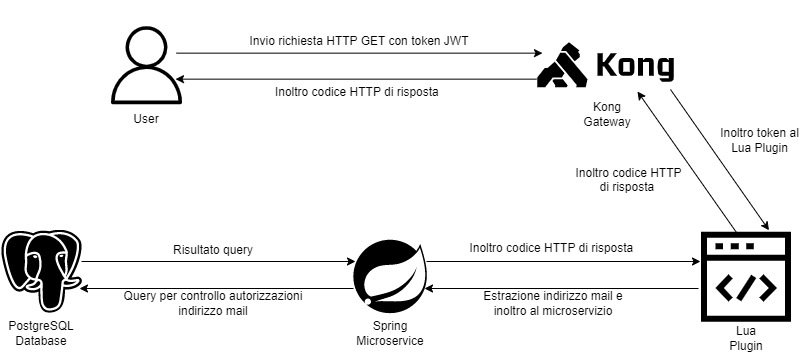
\includegraphics{img/comunicazioni_applicazioni.drawio.png}}
    \caption{Schema comunicazioni}
    \label{fig:comunicationscheme}
\end{figure}

Ricapitolando, dallo schema delle comunicazioni si evince che il funzionamento dell'applicazione si articola in:
\begin{enumerate}
\item Invio della richiesta \texttt{HTTP GET} dall'utente a Kong Gateway.
\item Inoltro del token all'interno della richiesta da Kong Gateway al plugin Lua.
\item Estrapolazione dell'indirizzo mail dal token ricevuto (verificandone anche l'integrità).
\item Richiesta \texttt{HTTP GET} dal plugin al microservizio Spring.
\item Operazioni per il collegamento al Database.
\item Esecuzione della query per verificare le autorizzazioni dell'indirizzo mail ricevuto.
\item Ottenimento del risultato della query.
\item Si rimanda l'informazione ottenuta effettuando il percorso inverso, fino a comunicarla all'utente. 
\end{enumerate}

\section{Casi d'uso}\label{sec:casiuso}
L'applicazione da realizzare risulta adatta per l'integrazione su tutte le piattaforme che offrano dei servizi gratuiti e a pagamento, infatti, lo scopo è quello di 
determinare quali utenti di un'eventuale piattaforma siano autorizzati ad accedere a determinati servizi.\\ \\
Un reale esempio di applicazione del prodotto può essere una piattaforma che fornisca servizi di PEC (Posta Elettronica Certificata) ma anche di fatturazione elettronica.\\
Si supponga che l'utilizzo della PEC sia gratuito per tutti gli utenti registrati, mentre la fatturazione elettronica sia riservata ai soli utenti che abbiano sottoscritto 
un abbonamento: in questo caso il prodotto realizzato soddisferebbe la necessità di controllare a quali livelli della piattaforma un determinato utente ha il permesso di accedere.

\chapter{Progettazione e sviluppo}\label{chapter:progettazionesviluppo}
In questo capitolo saranno esposti gli approcci teorici e pratici per lo sviluppo del progetto.


\section{Introduzione ai microservizi}\label{sec:microserviziintro}
Prima di introdurre il concetto di architettura a microservizi è bene introdurre il concetto di architettura monolitica.\\
Un'architettura monolitica è una metodologia di sviluppo secondo la quale tutti i processi coinvolti sono strettamente legati tra di loro e sono erogati 
come un singolo servizio.\\
Questa tipologia di approccio porta ad avere sistemi nei quali modificare le funzionalità diventa più complesso in quanto si deve agire sull'intero sistema e non 
solo sulle parti effettivamente interessate.\\
Inoltre, utilizzare un'architettura monolitica porta a correre dei rischi per quanto riguarda la disponibilità dell'applicazione, in quanto anche se solo uno dei 
processi coinvolti avesse un malfunzionamento, questo si propagherebbe nell'intera applicazione.\\ \\
Per quanto riguarda le architetture a microservizi, queste sono diametralmente opposte alle architetture monolitiche.\\
Nelle architetture a microservizi l'obiettivo è quello di scomporre l'applicazione da realizzare nelle sue funzioni (\emph{servizi}) di base.\\
Ogni servizio può essere compilato e distribuito in modo indipendente; quindi i singoli servizi possono funzionare o non funzionare senza compromettere gli altri.\\
Utilizzare i microservizi significa riuscire a gestire criticità inevitabili, poter sfruttare la scalabilità dinamica e semplificare l'integrazione 
di nuove caratteristiche. \cite{RedHatMicroservices}, \cite{Amazon}\\

\begin{figure}[ht]
	\centering
	\resizebox{1.0\textwidth}{!}{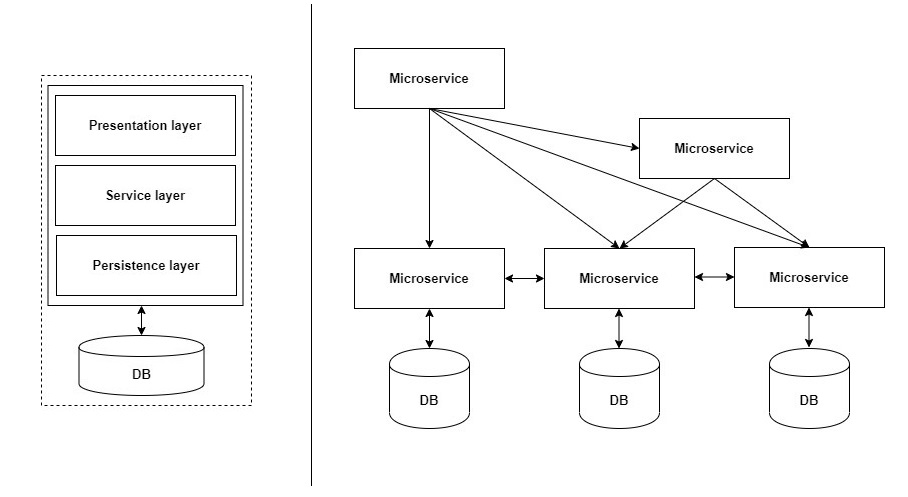
\includegraphics{img/monovsmicro}}
	\caption{Architettura monolitica e architettura a microservizi a confronto}
	\label{fig:one}
\end{figure}

Oggi i container Linux permettono di eseguire più parti di un'applicazione in modo indipendente con un controllo superiore sui singoli componenti.\\
I microservizi containerizzati rappresentano la base delle applicazioni cloud native. \cite{RedHatDocker}\\ \\
Di seguito sono elencati alcuni dei vantaggi di un'architettura a microservizi:

\begin{itemize}
	\item \textbf{Agilità}\\ Essendo ogni applicazione suddivisa in servizi di base, i team di sviluppo agiscono in contesti ridotti, semplificando il lavoro e riducendo i tempi del ciclo di sviluppo.
	\item \textbf{Scalabilità}\\Lavorare con un microservizio consente di scalare in modo indipendente per rispondere alla richiesta di un determinato servizio.\\ In questo modo è possibile misurare il carico di lavoro di un singolo servizio e adattarlo di conseguenza; il che può portare a dei vantaggi anche in termini economici per il mantenimento dell'applicazione. 
	\item \textbf{Semplicità di distribuzione}\\ I microservizi supportano l'approccio \emph{CI/CD} (Continuous Integration/Continuous Delivery), così da semplificare l'integrazione e il testing di nuove funzionalità avendo comunque la possibilità di effettuare un rollback in caso di problemi.
	\item \textbf{Codice riutilizzabile}\\ Uno dei vantaggi del suddividere un'applicazione in servizi è la possibilità di poter riutilizzare codici di servizi già esistenti per altre applicazioni.
	\item \textbf{Resilienza}\\ Avendo un'applicazione a servizi indipendenti si aumenta la resilienza in caso di errori.\\ Si possono gestire completamente gli errori di un servizio isolando la funzionalità senza bloccare l'intera applicazione.
\end{itemize}

\section{Il microservizio \texttt{CheckEmail}}\label{sec:architetturamicroservizio}
Il microservizio realizzato verifica l'avvenuto acquisto di un modulo applicativo da parte di un utente identificato, ai fini del microservizio, tramite un indirizzo e-mail.\\
Lo scopo principale del microservizio è quello di ricevere una richiesta \texttt{HTTP} con all'interno del body un indirizzo e-mail.\\
Una volta estratto l'indirizzo e-mail il microservizio effettua una \emph{query} all'interno del Database per controllare che l'indirizzo sia presente nella tabella degli utenti abilitati all'utilizzo di un determinato servizio.\\
In base al risultato della query il microservizio restituisce un codice \texttt{HTTP} come risposta alla richiesta.\\
\newline
La tipologia di richieste descritte sono effettuate tramite il metodo \textbf{\texttt{GET}} di \texttt{HTTP}, quindi vengono richiesti dei dati dal server.\\
\newpage
I codici che possono essere restituiti sono:\\
\begin{table}[ht]
	\centering
	\resizebox{1.0\linewidth}{!}{
		\begin{tabularx}{\linewidth}{|>{\centering\arraybackslash}m{3cm}|>{\centering\arraybackslash}m{4cm}|>{\centering\arraybackslash}m{5cm}|}
			\hhline{|-|-|-|}
			\textbf{Codice HTTP} & \textbf{Significato} & \textbf{Descrizione}\\
			\hhline{|-|-|-|}
			200 & OK & Il microservizio ha risposto correttamente e l'utente è autorizzato a procedere. \\
			\hhline{|-|-|-|}
			402 & PAYMENT REQUIRED & Il microservizio ha risposto correttamente ma l'utente non è autorizzato a procedere.\\
			\hhline{|-|-|-|}
			500 & INTERNAL SERVER ERROR & Messaggio di errore generico, non si è potuto raggiungere il microservizio.\\
			\hhline{|-|-|-|}
			503 & SERVICE UNAVAILABLE & Server non disponibile, non si è potuto raggiungere il microservizio. \\
			\hhline{|-|-|-|}
		\end{tabularx}
	}
	\vspace*{6mm}
	\caption{Codici HTTP restituiti dal microservizio}
	\label{tab:httpcode}
\end{table}

\begin{figure}[ht]
	\centering
	\resizebox{0.9\textwidth}{!}{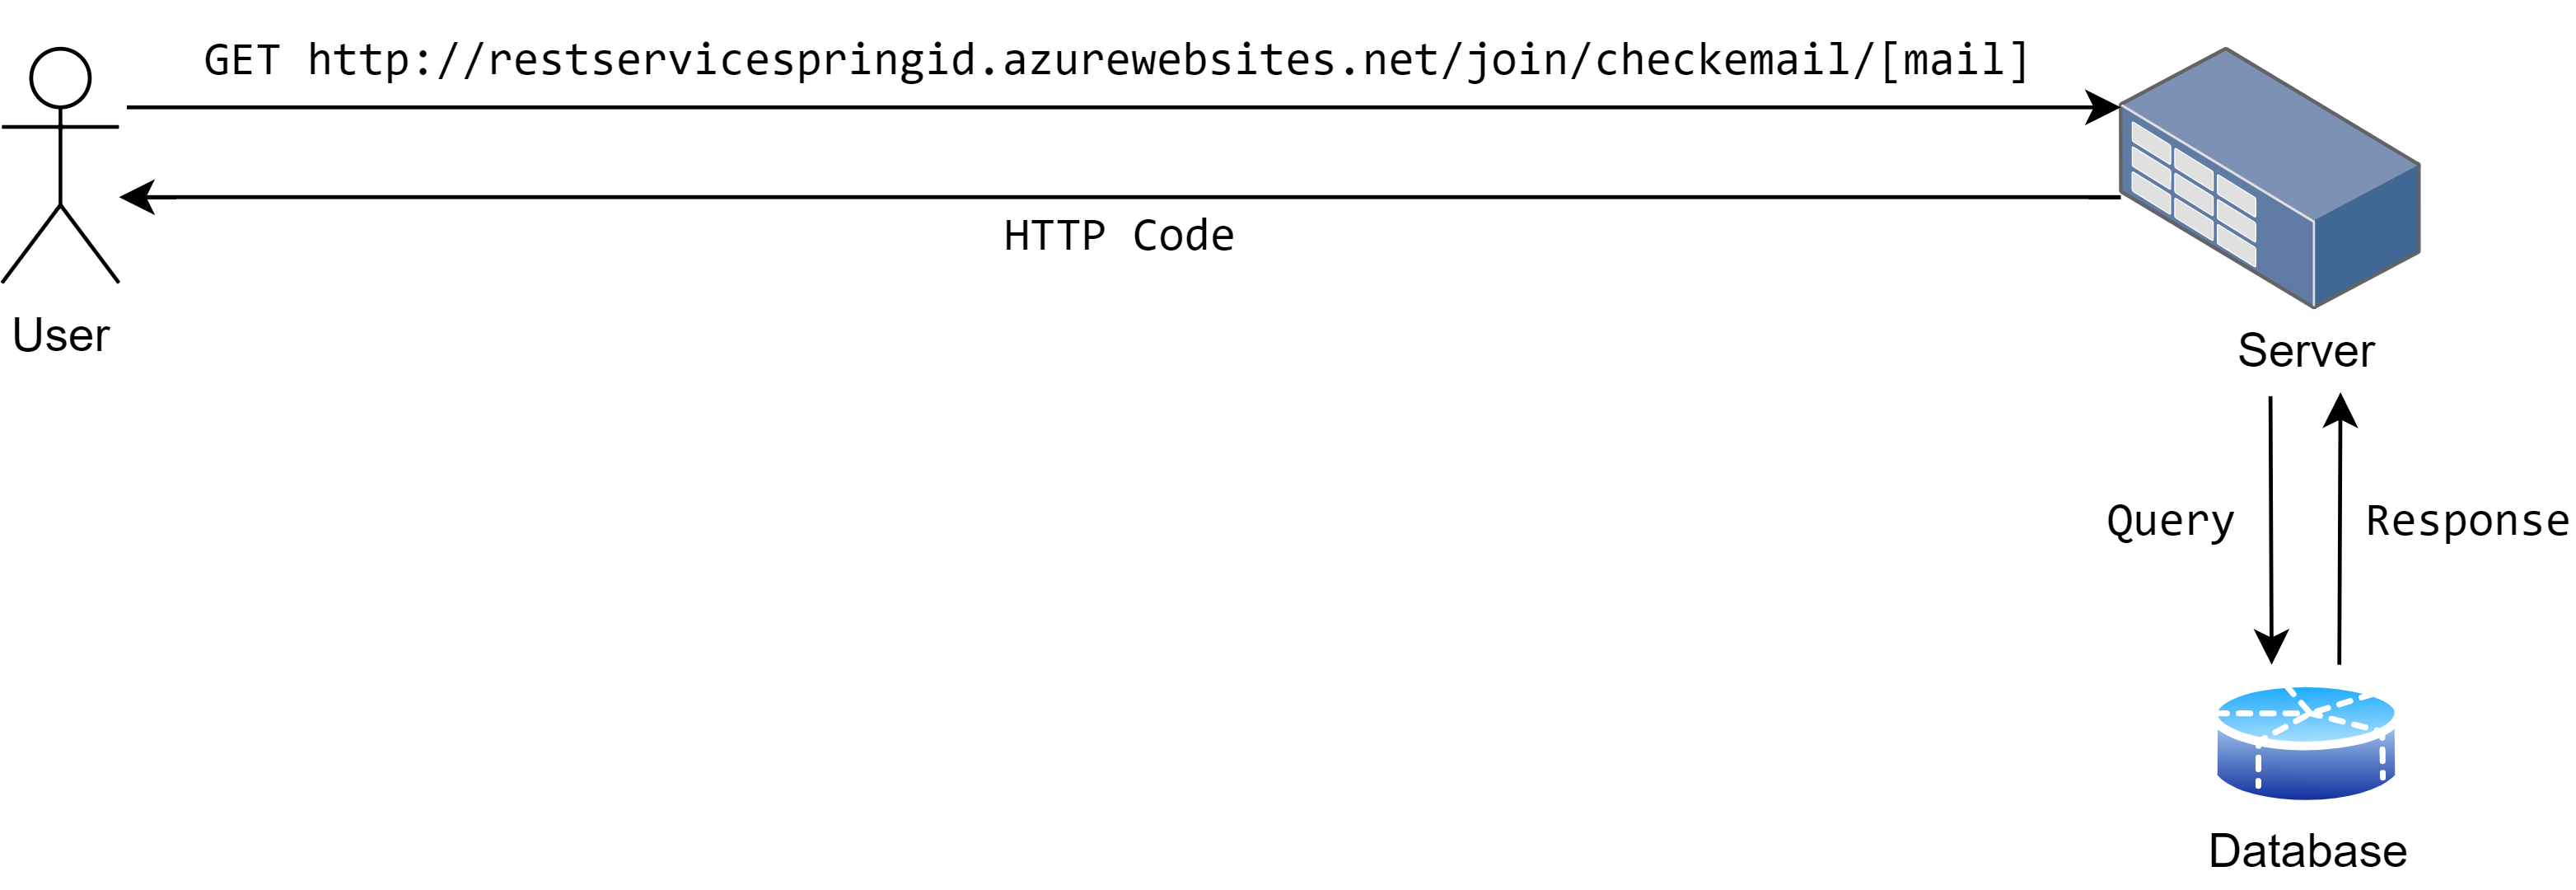
\includegraphics{img/comunicazionemicroservizio}}
	\caption{Schema di comunicazione Utente - microservizio}
	\label{fig:one}
\end{figure}

\subsection{Sviluppo}\label{sec:sviluppomicroservizio}
\subsubsection{Database}
Per sviluppare ed utilizzare il microservizio si è resa necessaria la creazione del Database PostgreSQL per la memorizzazione dei dati degli utenti.\\
È bene premettere che il Database è stato volutamente creato nella maniera più semplice e facilmente manutenibile, dato che durante lo sviluppo questo doveva servire solo per scopi di testing.\\
Il Database è composto da due tabelle:
\begin{itemize}
		\item \textbf{\texttt{users}}\\ Contiene le informazioni di tutti gli utenti abilitati ad accedere ad un determinato servizio.
		\item \textbf{\texttt{email}}\\ Contiene gli indirizzi e-mail di tutti gli utenti della piattaforma, quindi non è garantito che tutti avranno accesso a tutti i servizi.
\end{itemize}
\begin{figure}[ht]
	\centering
	\resizebox{0.3\textwidth}{!}{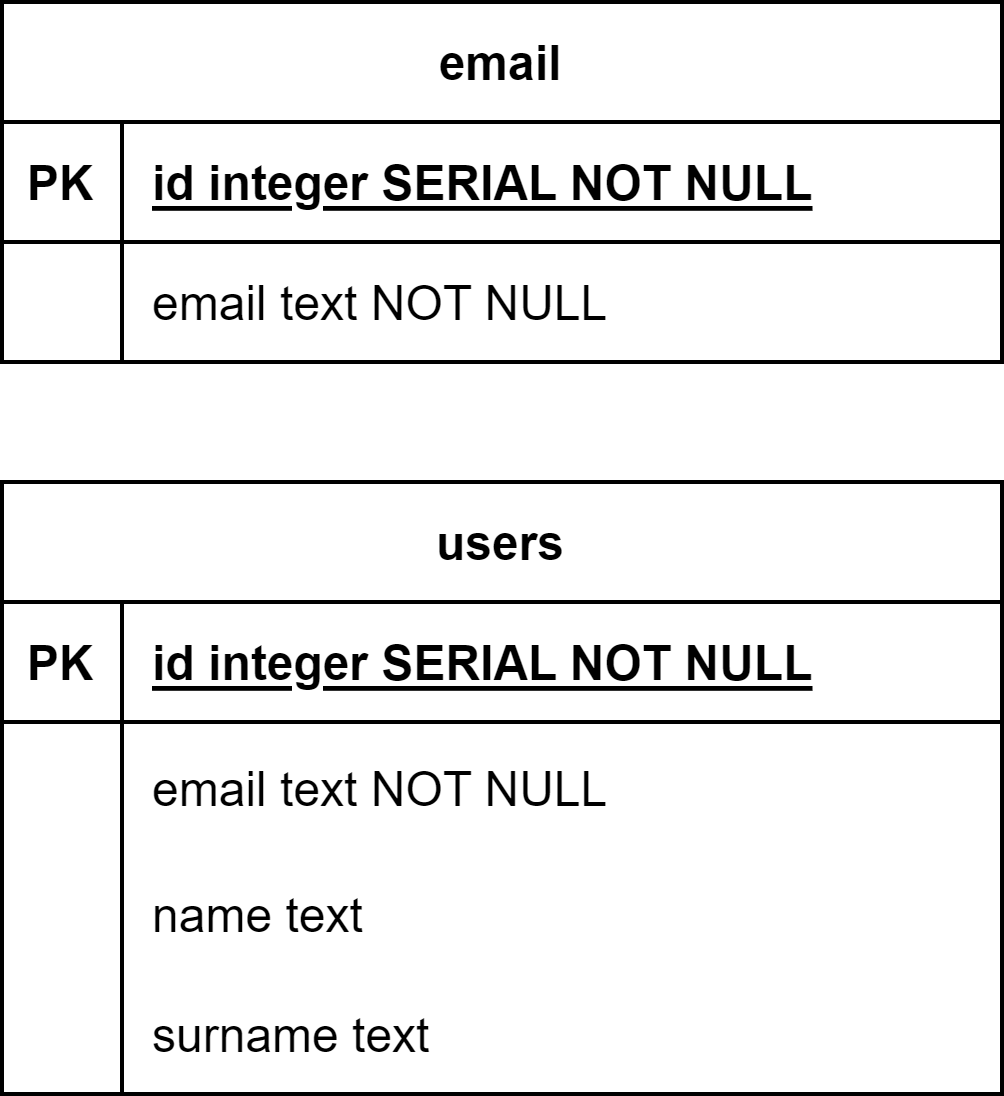
\includegraphics{img/dbtables-drawio}}
	\caption{Modello Entità Relazione del Database}
	\label{fig:one}
\end{figure}

\begin{figure}[ht]
	\centering
	\resizebox{0.7\textwidth}{!}{\includegraphics{img/emaildb_e}}
	\caption{Contenuto delle tabelle visualizzato dalla shell di PostgreSQL}
	\label{fig:one}
\end{figure}

\subsubsection{Microservizio}
Per lo sviluppo del microservizio, come accennato in precedenza, è stato deciso di utilizzare il linguaggio di programmazione Java e il framework Spring.\\
Il progetto è stato realizzato utilizzando l'IDE Eclipse ed è composto da cinque \emph{package}.
\begin{figure}[h]
	\centering
	\resizebox{0.6\textwidth}{!}{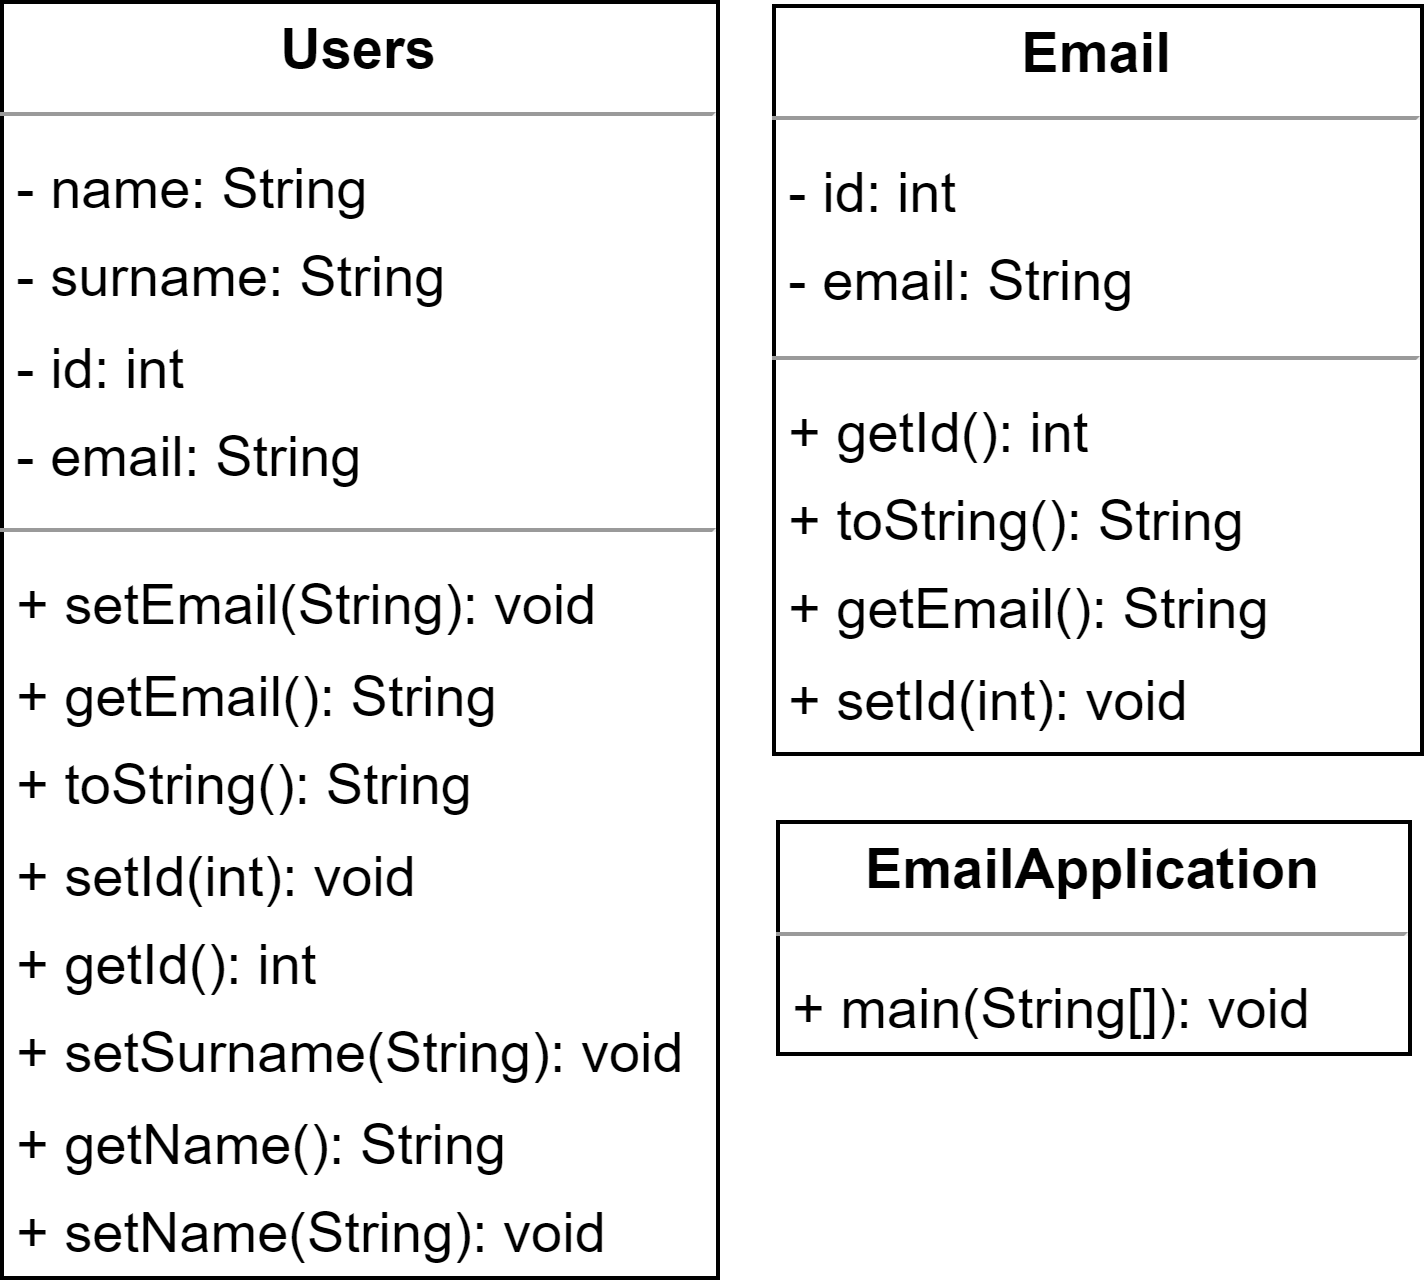
\includegraphics{img/classi}}
	\caption{Diagramma UML delle classi principali del progetto}
	\label{fig:one}
\end{figure}

\begin{figure}[h]
	\centering
	\resizebox{0.8\textwidth}{!}{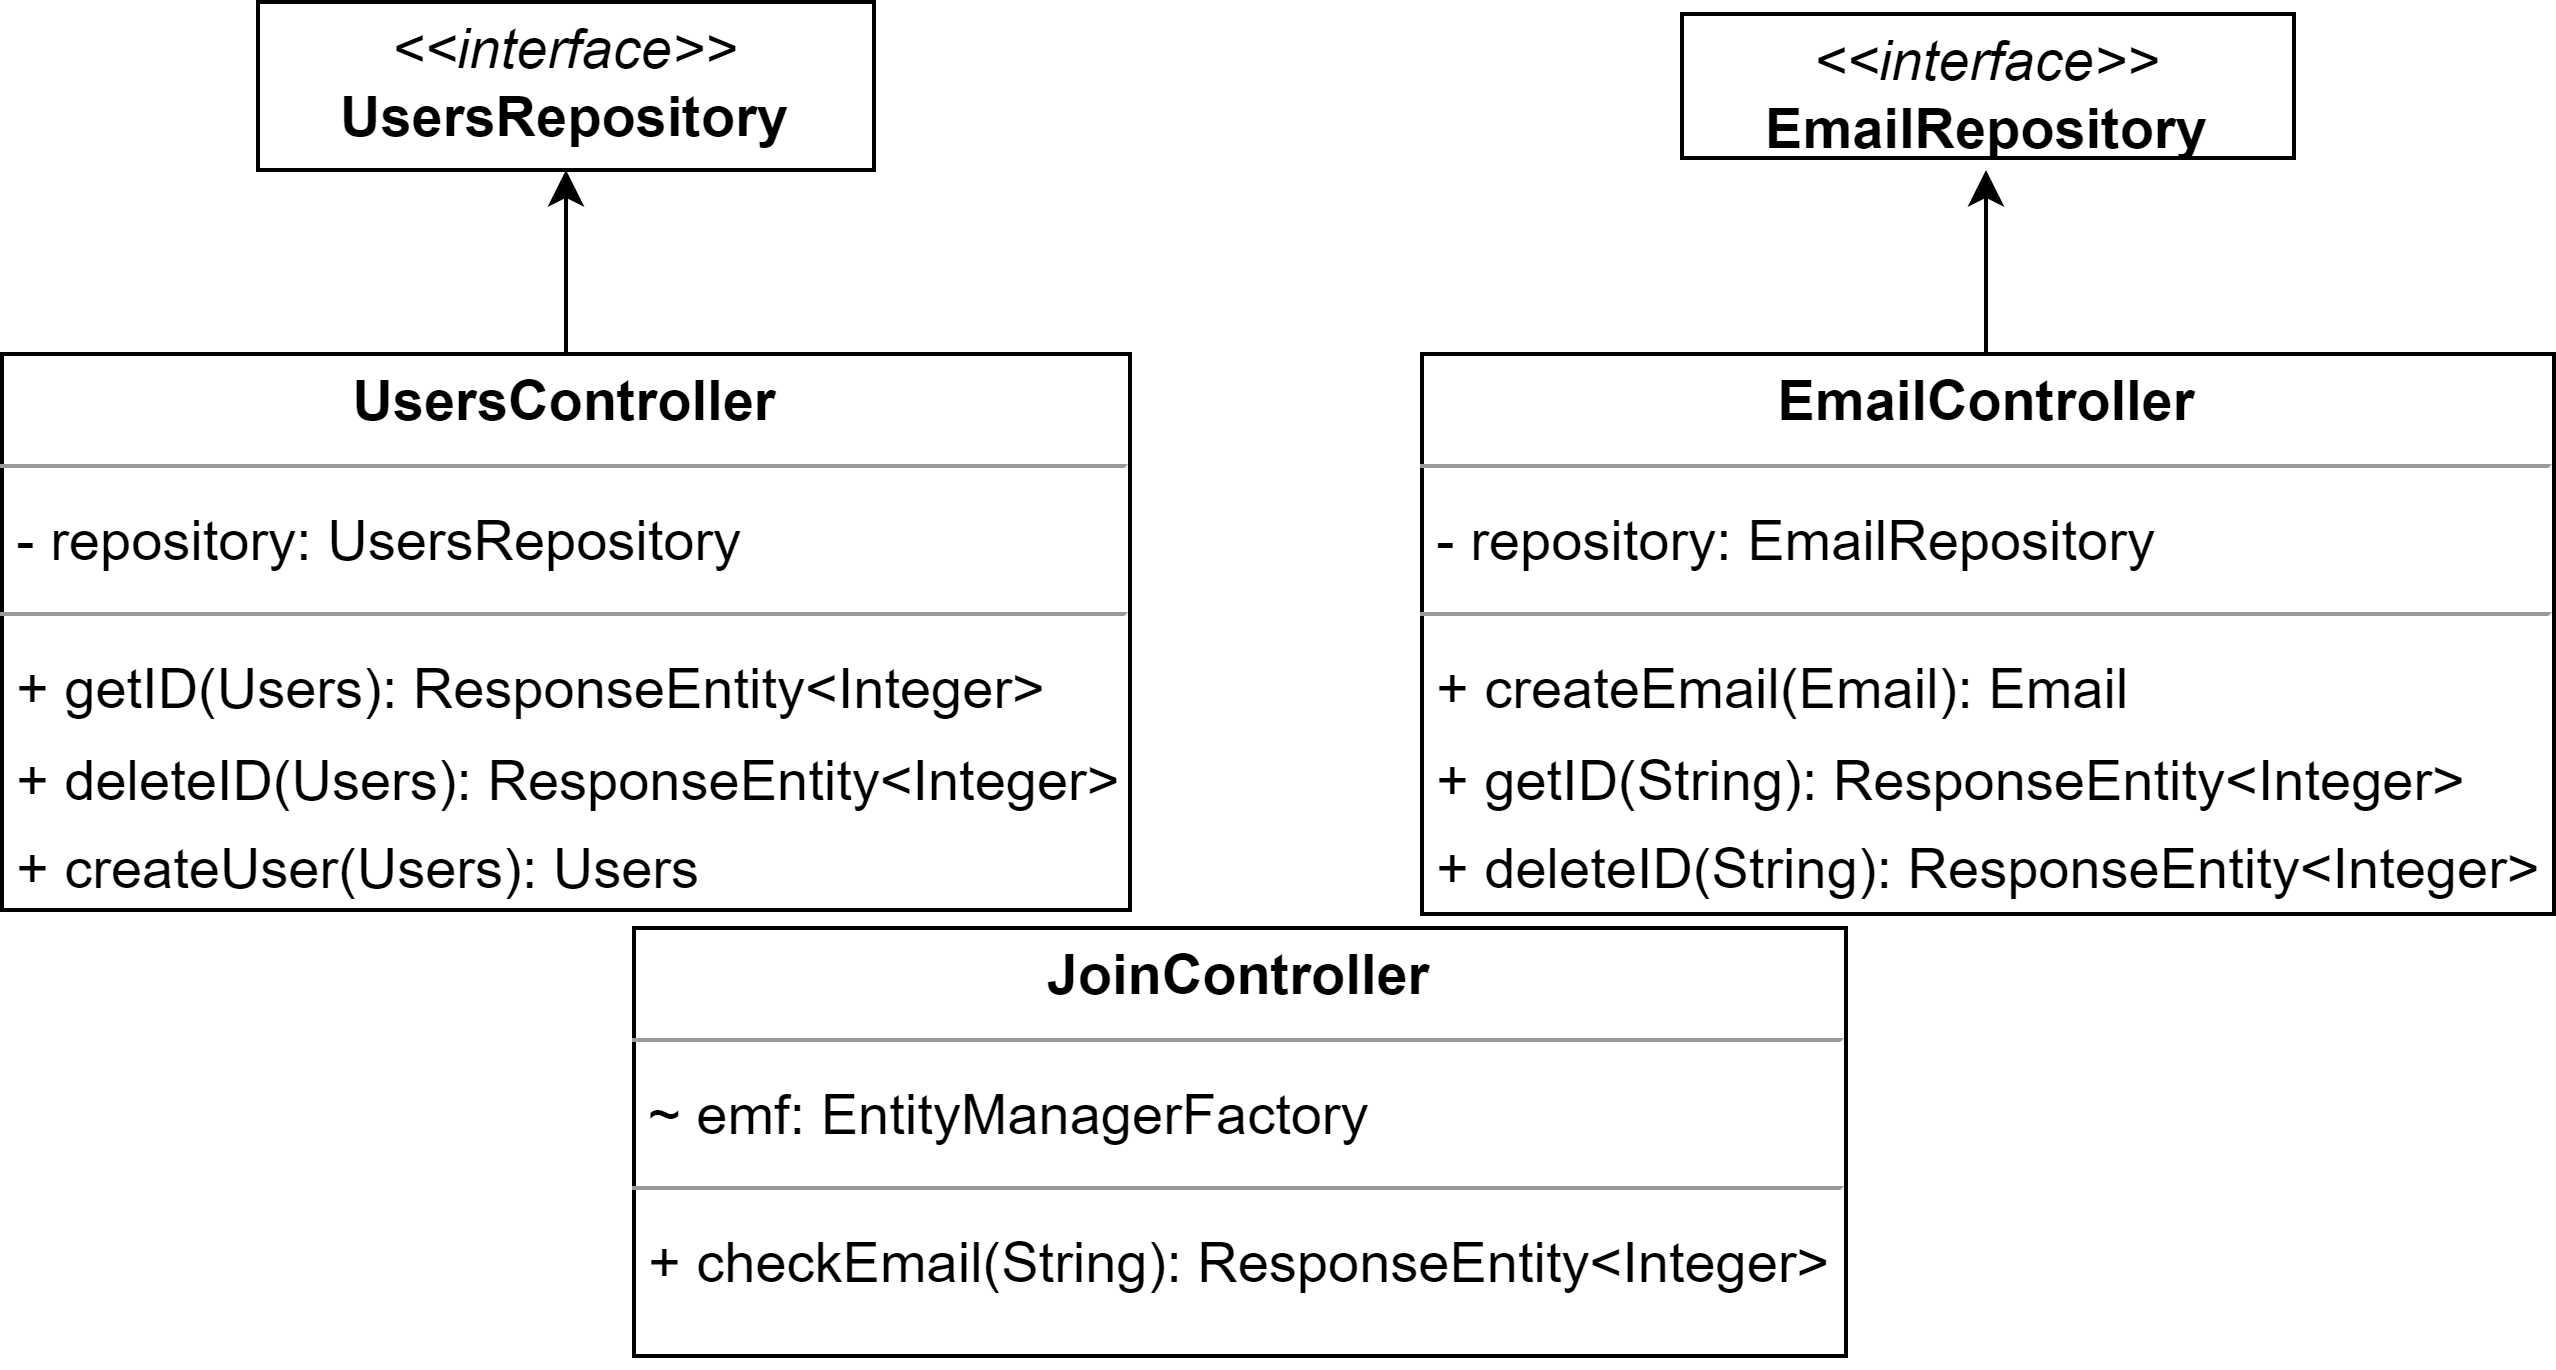
\includegraphics{img/controller}}
	\caption{Diagramma UML delle classi \emph{controller} del progetto}
	\label{fig:one}
\end{figure}
\newpage
\begin{figure}[h]
	\centering
	\resizebox{0.5\textwidth}{!}{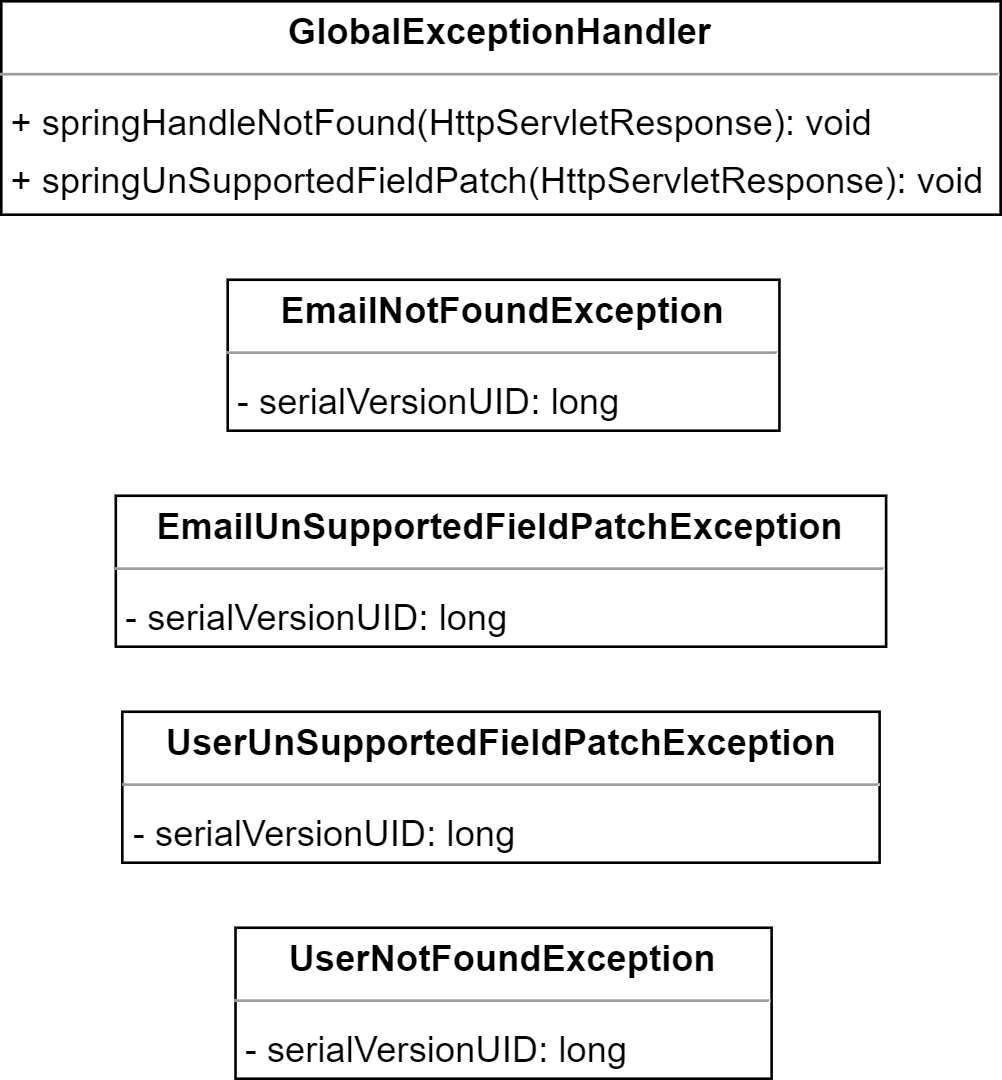
\includegraphics{img/exception}}
	\caption{Diagramma UML delle \emph{custom exception} del progetto}
	\label{fig:one}
\end{figure}

Descrizione dei package:
\begin{itemize}
	\item \textbf{\texttt{com.aesys.valeriodesiati.mail}}\\ Contiene la classe principale del microservizio.
	\item \textbf{\texttt{com.aesys.valeriodesiati.mail.model}}\\ Contiene le classi relative alle Entità all'interno del Database.\\ \emph{Spring Boot JPA} consente la creazione di entità in un Database a partire da una normale classe Java tramite l'aggiunta di annotazioni fornite dal framework.\\Un esempio di utilizzo di un \emph{model} è l'Algoritmo \ref{alg:checkemailmodel}.\\Il risultato sarà quindi la creazione di una tabella nel Database con i campi specificati dalle relative variabili annotate.
	\item \textbf{\texttt{com.aesys.valeriodesiati.mail.repository}}\\ Contiene le interfacce relative alle entità del Database che ereditano l'interfaccia \mintinline{java}{JpaRepository<T,ID>}.\\ Tale interfaccia contiene le API per tutte le operazioni CRUD di base.\\ CRUD (Create Read Update Delete) è un acronimo che indica le quattro operazioni fondamentali per creare un'applicazione che abbia uno storage persistente.
	\item \textbf{\texttt{com.aesys.valeriodesiati.mail.controller}}\\ Contiene le classi \emph{Controller} del microservizio, ovvero le classi annotate con \mintinline{java}{@RestController}.\\ In Spring una classe annotata come \emph{Controller} è una classe che sarà utilizzata come handler di richieste web.\\Un esempio di utilizzo di un \mintinline{java}{@RestController} è l'Algoritmo \ref{alg:checkemail}.
	\item \textbf{\texttt{com.aesys.valeriodesiati.mail.exception}}\\ Contiene le classi per la definizione di \emph{custom exception}.\\ L'implementazione di tali classi si è resa necessaria per poter comprendere meglio gli errori in fase di sviluppo e di debug.\\
\end{itemize}

\begin{algorithm}
\centering
\begin{minted}[fontsize=\scriptsize, xleftmargin=20pt,linenos]{java}
@Entity
@Table (name="email")
public class Email {

	@Id
	@GeneratedValue(strategy=GenerationType.IDENTITY)
	private int id;
	@Column(name = "email")
	private String email;
	
	public Email() {}

	public Email(int id, String email) {
		this.id = id;
		this.email = email;
	}
	
	//getters, setters and toString()...
}
\end{minted}
\caption{Utilizzo di un \emph{model} di Spring Boot JPA}\label{alg:checkemailmodel}
\end{algorithm}

\begin{algorithm}
\centering
\begin{minted}[fontsize=\scriptsize, xleftmargin=20pt, linenos]{java}
	@Transactional
	@GetMapping("/join/checkemail/{mail}")
	public ResponseEntity<Integer> checkEmail(@PathVariable("mail") String mail) {

	EntityManager em = emf.createEntityManager();
	em.getTransaction().begin();
	String result = null;

	try {
		result = (String) em.createQuery("SELECT u.email
                                                  FROM Users u, Email e
                                                  WHERE u.email = e.email 
                                                  AND u.email = :email")
                                                  .setParameter("email", mail)
                                                  .getSingleResult();
	}
	catch(NoResultException | NullPointerException e) {
		return ResponseEntity.status(HttpStatus.PAYMENT_REQUIRED).body(402);
	}

	if(result == null)
		return ResponseEntity.status(HttpStatus.PAYMENT_REQUIRED).body(402);
	else
		return ResponseEntity.status(HttpStatus.OK).body(200);

	}
\end{minted}
\caption{Accesso al Database}\label{alg:checkemail}
\end{algorithm}

Andando ad analizzare più a fondo le specifiche dell'Algoritmo \ref{alg:checkemail} è possibile notare, in testa al metodo, l'annotazione\\ \\
\centerline{\mintinline{java}{@GetMapping("/join/checkemail/{mail}")}} \\ \\
tramite la quale diventa possibile intercettare delle richieste \texttt{HTTP GET} effettuate in un determinato percorso. Il parametro \mintinline{java}{{mail}} può essere
utilizzato all'interno della funzione.\\
Si passa poi alla creazione di un \mintinline{java}{EntityManager} che consente di eseguire query all'interno delle \emph{entity} create tramite i \emph{model}.\\ \\
I passaggi successivi sono per la creazione e l'esecuzione della query, che effettua un'operazione di join tra le tabelle \texttt{Users} e \texttt{Email}, andando
semplicemente a controllare che l'indirizzo mail specificato nella richiesta \texttt{HTTP GET} sia effettivamente presente all'interno della tabella \texttt{Users} e
quindi sia abilitato all'accesso.\\
Il tutto è svolto all'interno di un blocco \mintinline{java}{try{ } catch(Exception){ }} al fine di prevenire comportamenti anomali: se viene lanciata l'eccezione\\
\mintinline{java}{NoResultException} o \mintinline{java}{NullPointerException}, si ritorna il codice \texttt{HTTP 402 Payment Required}.
Se si termina l'esecuzione della query senza eccezioni e la variabile \mintinline{java}{result} non è impostata a \mintinline{java}{null}, si ritorna il codice \texttt{HTTP 200 OK}.


% \begin{figure}[ht]
% 	\centering
% 	\resizebox{1.0\textwidth}{!}{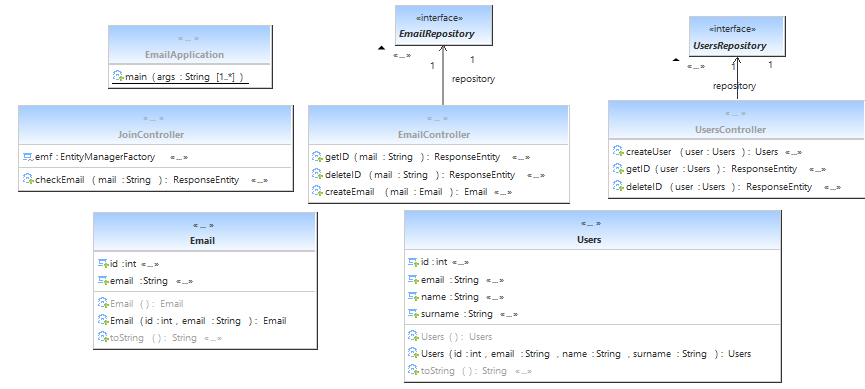
\includegraphics{img/uml}}
% 	\caption{Schema di comunicazione Utente - microservizio}
% 	\label{fig:one}
% \end{figure}

\section{Introduzione a Kong Gateway}\label{sec:kongprog}
Come accennato nel paragrafo \ref{sec:kongintro}, \emph{Kong Gateway} è un API gateway cloud-native che fornisce l'opportunità di configurare \emph{services} e \emph{routes} e, oltre a questi, anche \emph{plugin} e \emph{consumer}.
\subsection{Service}\label{sec:kongservice}
Un \emph{service} in Kong Gateway è un'astrazione di tutti i servizi upstream custom che si aggiungono alla configurazione. Con \emph{servizio upstream custom} si intende un microservizio custom che prende dati dalla richiesta inoltrata al gateway e ne restituisce altri al gateway stesso, che si occuperà di comunicarli al client.\\
Solitamente ad ogni \emph{service} è associata una o più \emph{routes}. \cite{Kong}\\

\subsection{Route}\label{sec:kongroute}
Una \emph{route} è una regola definita per indirizzare correttamente le richieste del client.\\
L'associazione di una (o più) route ad un servizio consente di realizzare un meccanismo di routing molto potente, dato che è possibile configurare
 nel dettaglio il percorso che si vuole realizzare (protocolli da utilizzare, livello di sicurezza ecc.). \cite{Kong}\\

\subsection{Consumer}\label{sec:kongconsumer}
Un \emph{consumer} in Kong Gateway può essere inteso come un utente di uno specifico servizio e può essere identificato tramite un \texttt{id} univoco. \cite{Kong}

\subsection{Plugin}\label{sec:kongplugin}
Un \emph{plugin} è un'entità che sarà eseguita durante tutto il ciclo di vita di una richiesta o risposta HTTP/S (HyperText Trasfer Protocol / Secure).\\
È il modo in cui Kong Gateway fornisce la possibilità di ottenere funzionalità aggiuntive per un \emph{service} o una \emph{route}.\\
I plugin configurabili possono essere sia proprietari (attivabili da Kong Manager) sia custom. Per la realizzazione di un plugin custom si ha la possibilità 
di scegliere tra vari linguaggi di programmazione per lo sviluppo quali Go, Python, JavaScript e Lua (linguaggio utilizzato per lo sviluppo 
del plugin custom utilizzato nel progetto). \cite{Kong}\\ 

\section{Architettura del plugin \texttt{checkemail}}\label{sec:architetturaplugin}
Un plugin in Lua per Kong Gateway si compone principalmente di due file:

\begin{itemize}
	\item \textbf{\texttt{handler.lua}}\\ Questo file contiene tutta la logica del plugin, devono essere implementate tutte le funzioni coinvolte nel ciclo richiesta/risposta.
	\item \textbf{\texttt{schema.lua}}\\ Racchiude tutte le configurazioni addizionali, se necessarie, come ad esempio coppie chiave/valore o altre impostazioni per modificare il comportamento del plugin.
\end{itemize}

Il funzionamento e l'utilizzo di questi file sarà approfondito nel paragrafo successivo e nel paragrafo \ref{sec:kongconf}.

\subsection{Sviluppo}\label{sec:sviluppoplugin}
Come detto in precedenza la logica del plugin è interamente contenuta nel file \texttt{handler.lua}.\\ 
È richiesto il seguente comportamento dal plugin:

\begin{enumerate}
	\item Analizzare il token ricevuto.
	\item Parse del token.
	\item Inviare una richiesta \texttt{HTTP} al microservizio \texttt{CheckEmail}.
	\item Ottenere e inoltrare al Gateway il codice di risposta ottenuto.
\end{enumerate}

Il primo punto è realizzato dalla funzione \mintinline{lua}{SplitToken(token)}, che analizza il token \texttt{JWT} ricevuto e lo suddivide nelle tre parti di cui è composto: Header, Body e Signature.\\
La funzione restituisce un array contenente le tre componenti del token.

\begin{algorithm}
\centering
\begin{minted}[fontsize=\scriptsize, xleftmargin=20pt, linenos]{lua}
	local function SplitToken(token)
		local segments = {}
		for str in string.gmatch(token, "([^\\.]+)") do
			table.insert(segments, str)
		end
		return segments
	end
\end{minted}
\caption{Suddivisione token JWT}\label{alg:splittoken}
\end{algorithm}

Successivamente si procede con il parse del token, mediante la funzione \mintinline{lua}{ParseToken(token)} che inizia chiamando la funzione \mintinline{lua}{SplitToken(token)}
per ottenere l'array delle parti, per poi proseguire applicando una decodifica ad ogni parte controllando anche l'eventuale presenza di errori.\\
La funzione può restituire tre o quattro risultati: nel caso in cui non ci siano stati errori vengono restituite solo le tre componenti del token decodificate, altrimenti 
vengono restituiti quattro risultati, i primi tre impostati a \mintinline{lua}{null} (rappresentano i campi del token) e il quarto come stringa con un messaggio di errore.\\
Da notare come tutte le parti vengano prima suddivise e poi decodificate anche se il dato ricercato (l'indirizzo mail) si trova solo nel Body, questo per favorire e semplificare 
la ricerca di eventuali componenti del token corrotte.

\begin{algorithm}
\centering
\begin{minted}[fontsize=\scriptsize, xleftmargin=20pt, linenos]{lua}
	local function ParseToken(token)
		local segments = SplitToken(token)
		if #segments ~= 3 then
			return nil, nil, nil, "Invalid token"
		end

		local header, err = cjson_safe.decode(basexx.from_url64(segments[1]))
		if err then
			return nil, nil, nil, "Invalid header"
		end

		local body, err = cjson_safe.decode(basexx.from_url64(segments[2]))
		if err then
			return nil, nil, nil, "Invalid body"
		end

		local sig, err = basexx.from_url64(segments[3])
		if err then
			return nil, nil, nil, "Invalid signature"
		end

		return header, body, sig
	end
\end{minted}
\caption{Parse token JWT}\label{alg:parsetoken}
\end{algorithm}
\newpage
Il ciclo del funzionamento del plugin termina quindi l'estrazione dell'indirizzo mail dal token decodificato e l'inoltro della richiesta \texttt{HTTP} al microservizio \texttt{CheckEmail}.\\
Il microservizio è raggiungibile al link\\ \texttt{ http://restservice-springid.azurewebsites.net/join/checkemail/}, \\unendo al link l'indirizzo mail che si desidera controllare.\\
\begin{algorithm}
\centering
\begin{minted}[fontsize=\scriptsize, xleftmargin=20pt, linenos]{lua}
    local body, code, headers, status = 
			http.request("http://restservice-springid.azurewebsites.net
				      /join/checkemail/"..bodyTok.email)
\end{minted}
\caption{Inoltro richiesta \texttt{HTTP} dal plugin}\label{alg:pluginhttprequest }
\end{algorithm}

\newpage
L'ultimo controllo che si effettua è quello sul codice di ritorno \texttt{HTTP} ricevuto dal microservizio, quindi si invia una risposta da Kong Gateway all'utente.

\begin{algorithm}
\centering
\begin{minted}[fontsize=\scriptsize, xleftmargin=20pt, linenos]{lua}
    if code == 200 then
        return kong.response.exit(200, "Success")
    end

    if code == 402 then
        return kong.response.error(402, "Payment Required")
    end

	--response codes 500 and 503...
\end{minted}
\caption{Inoltro risposta dal plugin a Kong Gateway}\label{alg:plugingatewayresponse}
\end{algorithm}

\section{Configurazione Kong Gateway}\label{sec:kongconf}
Kong Gateway è stato containerizzato tramite Docker utilizzando l'immagine ufficiale presente su Docker Hub.\\
Il container è stato reso raggiungibile tramite una macchina virtuale su Azure con immagine Debian.\\
Sono state create delle pipeline CI/CD per automatizzare i processi di containerizzazione e di installazione del plugin.\\
La pipeline è azionata automaticamente dai cambiamenti nella repository principale del progetto e si occupa di far eseguire, all'interno della macchina virtuale, uno script per l'aggiornamento dei \emph{services}, \emph{routes}, \emph{consumers}.\\

Il gateway può essere configurato in modi diversi:
Interfaccia grafica di Kong Manager, disponibile collegandosi da browser alla porta 8002 del container.
Tramite file JSON contenenti le informazioni necessarie che saranno aggiunte al file di configurazione principale (\texttt{kong.conf}), inoltrati con delle richieste \texttt{HTTP POST} verso il container in esecuzione.
\\
Come detto in precedenza, gli aspetti configurabili sono:
\begin{itemize}
	\item\emph{Services}
	\item\emph{Routes}
	\item\emph{Consumers}
	\item\emph{Plugin}
\end{itemize}

Ognuno con un file JSON di configurazione dedicato.\\
I plugin custom, come quello realizzato, non necessitano di un file di configurazione dedicato, è sufficiente copiare i file relativi nella directory\\
\texttt{/usr/local/share/lua/5.1/kong/plugins/nome\_plugin/} del container.\\

Tutta la configurazione è effettuata tramite lo script bash \texttt{addplugin} che ha i seguenti compiti:
\begin{itemize}
\item Avviare il container.
\item Copiare all'interno i file relativi ai plugin custom.
\item Riavviare il container (per consentire la lettura dei file dei plugin caricati)
\item Eseguire il comando \mintinline{bash}{curl} per tutti i file JSON presenti relativi a tutte le altre configurazioni necessarie.
\end{itemize}
Di seguito alcune righe dello script di configurazione:

\begin{algorithm}
\centering
\begin{minted}[fontsize=\scriptsize, xleftmargin=20pt, linenos]{sh}
    sudo docker exec -it --user root $container rm -rf 
				/usr/local/share/lua/5.1/kong/plugins/$dir
    sudo docker exec -it --user root $container mkdir
				/usr/local/share/lua/5.1/kong/plugins/$dir
    sudo docker cp . $container:/usr/local/share/lua/5.1/kong/plugins/$dir/
    curl -s -X POST -H "Content-Type: application/json"
	-d @./config/checkemail/services.json
	http://checkemail.westeurope.cloudapp.azure.com:8001/services > /dev/null
\end{minted}
\caption{Script per la configurazione di Kong Gateway}\label{alg:container_config}
\end{algorithm}


\chapter{Testing}

%
%
%%%% Le Conclusioni
\pagestyle{plain}
\chapter*{Conclusione} %Se si cambia il Titolo cambiare anche la riga successiva così che appia corretto nell'conclusione
\addcontentsline{toc}{chapter}{Conclusione} %Per far apparire Introduzione nell'indice (Il nome deve rispecchiare quello del chapter)
Al termine della realizzazione del progetto di stage tutti gli obiettivi descritti nel paragrafo \ref{sec:obiettivi} sono stati raggiunti nei tempi prefissati, 
secondo la ripartizione oraria riportata al paragrafo \ref{sec:ripartizionelavoro}.\\ \\

Il progetto, nella sua fase iniziale, non è risultato di semplice realizzazione in quanto è stato richiesto l'utilizzo di tecnologie e strumenti di cui non si era a conoscenza.\\ \\

Nel corso dello sviluppo ci sono state diverse problematiche:
\begin{itemize}
\item Immagini Docker.
\item Specifiche della Virtual Machine utilizzata.
\end{itemize}

All'inizio si era provato ad utilizzare l'immagine Docker \texttt{ubuntu:latest}, per poi decidere, in modo definitivo, di utilizzare l'immagine ufficiale di Kong Gateway 
per problemi di compatibilità e di raggiungibilità del Gateway.

Ancora, come spiegato nei capitoli precedenti, l'applicazione si trova all'interno di una Virtual Machine sulla quale è stato installato Docker con il relativo container Kong.\\
La problematica era relativa al fatto che in momenti completamente casuali l'applicazione risultava irraggiungibile, e quindi inutilizzabile.\\ 
Andando ad analizzare le statistiche di utilizzo su Microsoft Azure ci si è resi conto che il problema risiedeva nelle risorse (molto limitate) della Virtual Machine, 
che quindi accusava problemi di eccessivo utilizzo di CPU e RAM che implicava l'impossibilità di elaborare le richieste.\\ \\ 

Quindi, parlando di eventuali sviluppi futuri del progetto, sicuramente rientra tra questi il miglioramento delle specifiche della Virtual Machine da utilizzare,
 tenendo conto del fatto che le risorse a disposizione con l'attuale Virtual Machine sono 1 CPU e 512 MB di memoria RAM.\\
Altri sviluppi futuri potrebbero concentrarsi sull'implementazione di un Database più ampio e ottimizzato, andando ad utilizzare ad esempio Microsoft Azure SQL Database, 
il Database integrato nella piattaforma Azure.

%
%%%% La bibliografia
\nocite{*}
\bibliographystyle{unsrt} %{plain}
\addcontentsline{toc}{chapter}{Bibliografia}
\bibliography{Bibliografia}

% \nocite{*}
% \bibliographystyle{plain} %{apalike} -- Scegliere lo stile preferito
% \bibliography{./Bibliografia}
%
\chapter*{Ringraziamenti} %Se si cambia il Titolo cambiare anche la riga successiva così che appia corretto nell'conclusione
\addcontentsline{toc}{chapter}{Ringraziamenti} %Per far apparire Introduzione nell'indice (Il nome deve rispecchiare quello del chapter)
aaaaaaaaaaaaaaaaaaaaa
%
% Le appendici
\appendix
\chapter{Appendice}
\Blindtext
%
\end{document}